\documentclass[border=10pt]{standalone}
\usepackage[svgnames]{xcolor}
\usepackage{amsmath}
\usepackage{pgfplots}
\pgfplotsset{compat=newest}
\usepackage[sfdefault]{FiraSans}
\usepackage{FiraMono}
\renewcommand*\familydefault{\sfdefault}
\begin{document}
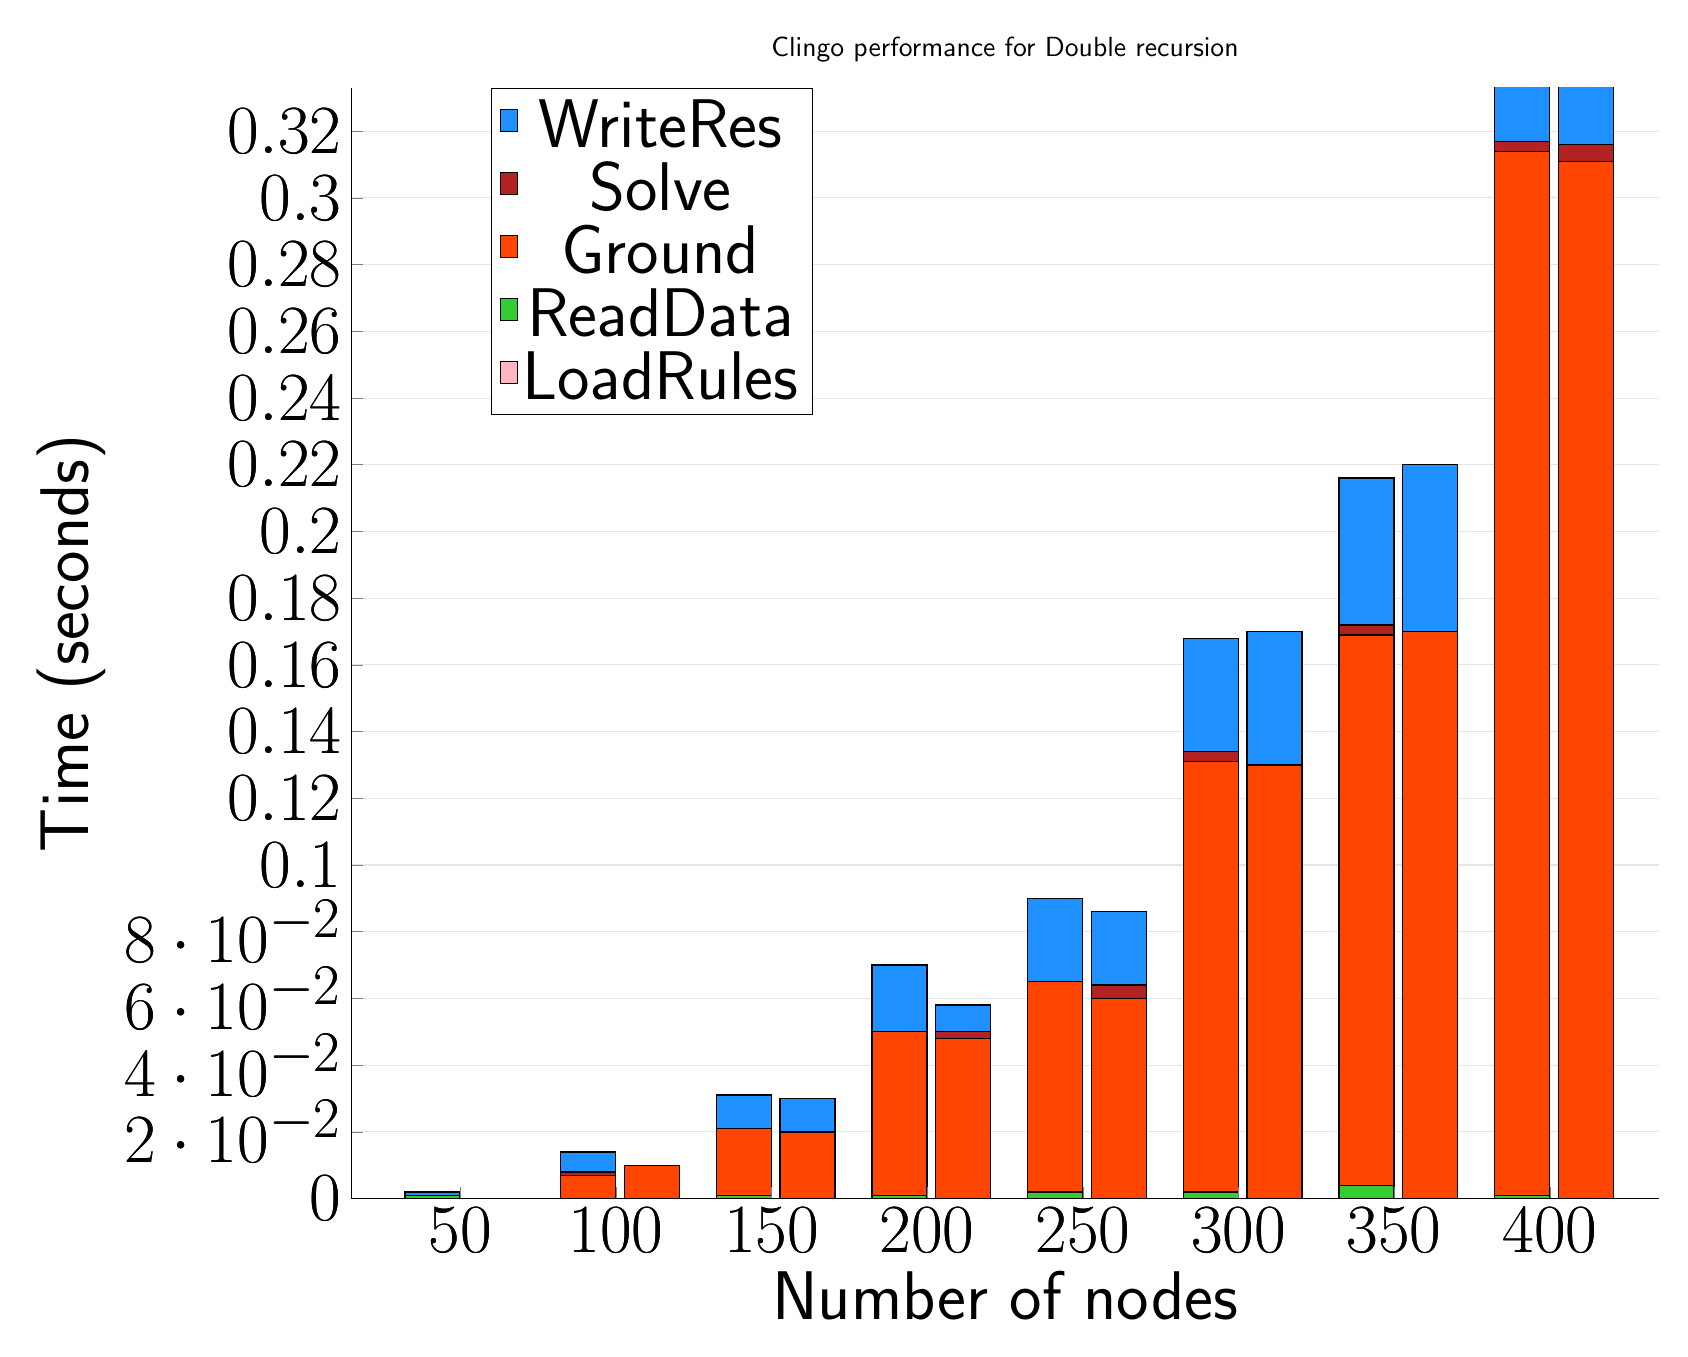
\begin{tikzpicture}
\begin{axis}[
   ybar stacked,
   title={Clingo performance for Double recursion},
   bar shift=-10pt,
   width=1.5\textwidth,
   bar width=0.7cm,
   ymajorgrids, tick align=inside,
   major grid style={draw=gray!20},
   xtick=data,
   ymin=0, ymax=0.3330000114440918,
   axis x line*=bottom,
   axis y line*=left,
   enlarge x limits=0.1,
   legend style={
       at={(0.23, 1)},
       anchor=north,
       legend columns=1,
       font=\Huge,
   },
   ylabel={Time (seconds)},
   xlabel={Number of nodes},
   label style={font=\Huge},
   tick label style={font=\Huge},
]
\addlegendimage{fill=DodgerBlue, draw=black, line width=0.2pt}
\addlegendentry{WriteRes}
\addlegendimage{fill=FireBrick, draw=black, line width=0.2pt}
\addlegendentry{Solve}
\addlegendimage{fill=OrangeRed, draw=black, line width=0.2pt}
\addlegendentry{Ground}
\addlegendimage{fill=LimeGreen, draw=black, line width=0.2pt}
\addlegendentry{ReadData}
\addlegendimage{fill=LightPink, draw=black, line width=0.2pt}
\addlegendentry{LoadRules}
\addplot +[fill=LightPink, draw=black, line width=0.5pt] coordinates {
    (50, 0.0)
    (100, 0.0)
    (150, 0.0)
    (200, 0.0)
    (250, 0.0)
    (300, 0.0)
    (350, 0.0)
    (400, 0.0)
};
\addplot +[fill=LimeGreen, draw=black, line width=0.5pt] coordinates {
    (50, 0.0009999990463256836)
    (100, 0.0)
    (150, 0.0009999990463256836)
    (200, 0.0009999990463256836)
    (250, 0.0019999980926513673)
    (300, 0.0020000219345092775)
    (350, 0.0039999961853027345)
    (400, 0.0009999990463256836)
};
\addplot +[fill=OrangeRed, draw=black, line width=0.5pt] coordinates {
    (50, 0.0)
    (100, 0.006999993324279785)
    (150, 0.020000004768371583)
    (200, 0.049000000953674315)
    (250, 0.06300005912780762)
    (300, 0.12899999618530272)
    (350, 0.16500003337860109)
    (400, 0.3130000114440918)
};
\addplot +[fill=FireBrick, draw=black, line width=0.5pt] coordinates {
    (50, 0.0)
    (100, 0.0009999990463256836)
    (150, 0.0)
    (200, 0.0)
    (250, 0.0)
    (300, 0.0029999971389770507)
    (350, 0.0029999971389770507)
    (400, 0.0029999971389770507)
};
\addplot +[fill=DodgerBlue, draw=black, line width=0.5pt] coordinates {
    (50, 0.0009999990463256836)
    (100, 0.005999994277954101)
    (150, 0.009999990463256836)
    (200, 0.02000002861022949)
    (250, 0.02499997615814209)
    (300, 0.03400001525878906)
    (350, 0.04399995803833008)
    (400, 0.06700000762939454)
};
\end{axis}
\begin{axis}[
   ybar stacked,
   bar shift=13pt,
   width=1.5\textwidth,
   bar width=0.7cm,
   ymajorgrids, tick align=inside,
   major grid style={draw=none},
   xtick=data,
   ymin=0, ymax=0.3330000114440918,
   axis x line*=none,
   axis y line*=none,
   enlarge x limits=0.1,
   label style={font=\Huge},
   tick label style={font=\Huge},
]
\addplot +[fill=LightPink, draw=black, line width=0.5pt] coordinates {
    (50, 0.0)
    (100, 0.0)
    (150, 0.0)
    (200, 0.0)
    (250, 0.0)
    (300, 0.0)
    (350, 0.0)
    (400, 0.0)
};
\addplot +[fill=LimeGreen, draw=black, line width=0.5pt] coordinates {
    (50, 0.0)
    (100, 0.0)
    (150, 0.0)
    (200, 0.0)
    (250, 0.0)
    (300, 0.0)
    (350, 0.0)
    (400, 0.0)
};
\addplot +[fill=OrangeRed, draw=black, line width=0.5pt] coordinates {
    (50, 0.0)
    (100, 0.009999999999999997)
    (150, 0.019999999999999997)
    (200, 0.047999999999999994)
    (250, 0.06000000000000001)
    (300, 0.12999999999999998)
    (350, 0.16999999999999998)
    (400, 0.31100000000000005)
};
\addplot +[fill=FireBrick, draw=black, line width=0.5pt] coordinates {
    (50, 0.0)
    (100, 0.0)
    (150, 0.0)
    (200, 0.0020000000000000018)
    (250, 0.003999999999999998)
    (300, 0.0)
    (350, 0.0)
    (400, 0.0050000000000000044)
};
\addplot +[fill=DodgerBlue, draw=black, line width=0.5pt] coordinates {
    (50, 0.0)
    (100, 0.0)
    (150, 0.010000000000000004)
    (200, 0.007999999999999998)
    (250, 0.022000000000000002)
    (300, 0.040000000000000015)
    (350, 0.04999999999999999)
    (400, 0.06499999999999997)
};
\end{axis}
\end{tikzpicture}

\end{document}
